% !TeX spellcheck = en_GB
% !TEX root = ../thesis-example.tex
%
\chapter{Evaluation \& future work}

\section{Hardware setup variations}

Due to the nature of this setup and fine-tweaking options inside the engine, 
this approach discussed can have a wide variety of operational setups. By lose 
coupling of these hardware factors there are only a few limitations that can 
either solved by better, future hardware or a different approach that are 
outside of the scope.

As integral part of this setup is the motion tracking solution, it is possible 
to hook up an Oculus Rift\footnote{with its room-scale setup} instead of the 
HTC Vive and set one controller as camera-attachment point. For that there 
would be another 3D print needed to attach the controller to a camera solution. 
\newline
Other third market VR-HMDs usually follow the Vives specifications closely and 
integrate natively with SteamVR, thus no modification on the original 
instalment has to be done.
\newline
Through Virtual Reality Peripheral Network or OpenVR simliar solutions can be 
developed, since none of the software explicitly depends on SteamVR features.

The other side, the video capture side, can be varied greatly too. Since the 
software only allows a webcam-compatible device, it would be possible to remove 
the Inogeni-Encoder and replace it with cheap and simple webcams. Similarly can 
a camera replaced along with other recording solutions, as long as it outputs 
an HDMI (or HDMI-convertible) video stream. This allows recording to be as 
complex as needed but in general a DSLR camera will suffice.

Finally, since the full pipeline is rather complex, a good desktop PC will be 
needed. The CPU overhead is minimal but the graphical complexity is based on 
limitations of the GPU. With future iteration of this hardware it will be 
possible to create more complex scenery.
\todo[inline]{you don't say >\_>}
In theory a low-poly environment could be render-able on mobile, combined with 
a low-sample rate on the camera image, to produce a "a window" into VR for 
multiple users at the same time, thus enabling an indefinite view into virtual 
reality. Further work could tap into a Microsoft HoloLens solution, which could 
enable a direct contextualization of an actor into a VR scenery. With fast 
approximate algorithms, like YCgCo-Keying, this could produce a high-framerate 
transparent overlay, so that the virtual scene does not clip the actor.
<<<<<<< Updated upstream
=======

While working with this setup another possible use-case showed up: On June 2017 
Apple presented their native Augmented Reality kit integrated in their consumer 
devices. Thus a similar setup could be used to send all tracking parameters 
from the HTC Vive headset to these devices and have a calibrated north-wall 
with additional feature markers. This would potentially allow to have an 
augmented reality view around the actors world with a fast approximated actor 
position. It could then be possible for multiple users to use these devices as 
window into the virtual reality experience.
>>>>>>> Stashed changes

\section{Rendering Setup Variations}

There are a few approaches that work similarly, but are different in 
complexity, their capabilities and hardware setups. They have been already 
explored and are covered here for completeness.

\subsection{Single Camera - 3D plane in space}

A novel approach is rendering the camera image onto a 2D plane positioned 
inside the 3D scene. This gives high control over projection parameters inside 
the engine without a running software and has good visual feedback for artists. 
All additional steps previously discussed are invalid, since this render can 
take full advantage of all realtime rendering parameters - which in turn means 
for lower render overhead and better graphical performance. It fails however on 
delay mitigation, which makes time drift between engine and camera visible, 
thus only usable with low latency video capturing devices.

\begin{figure}[htb]
	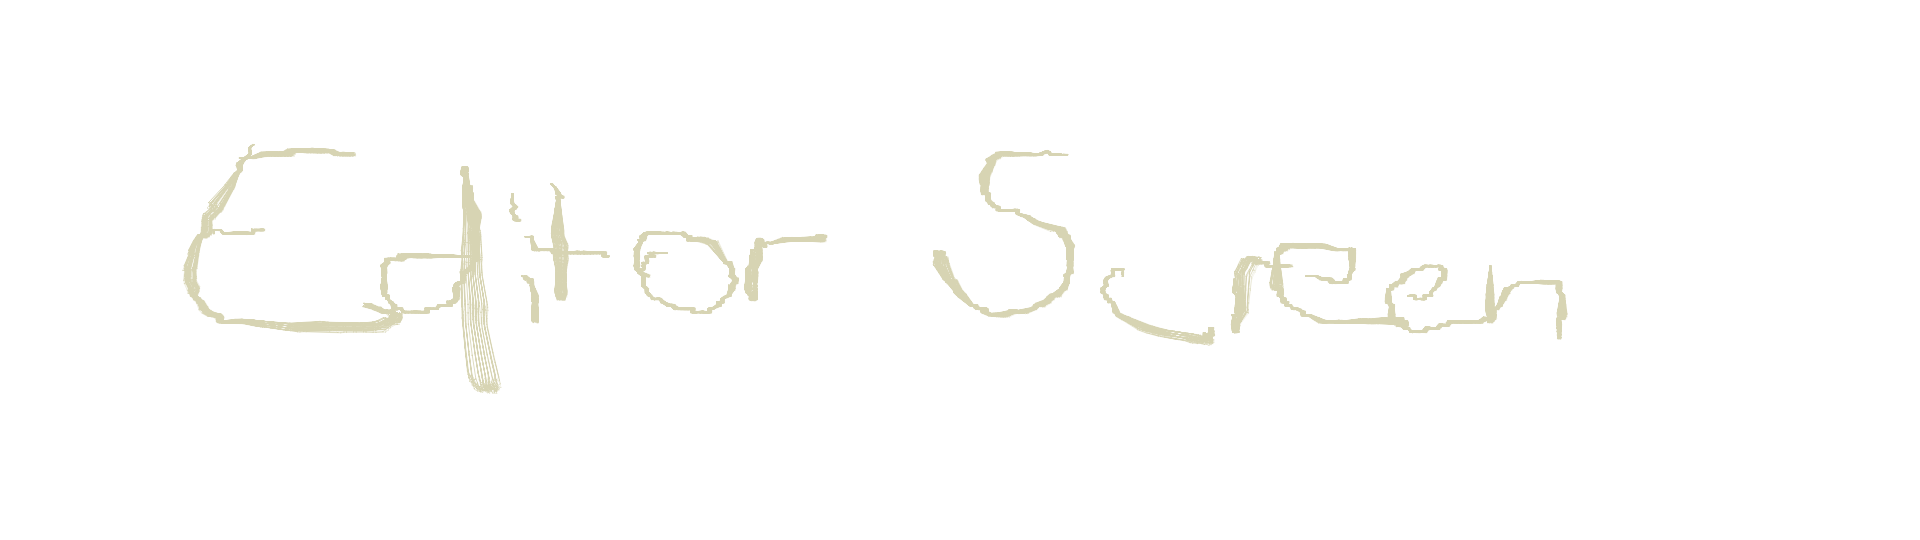
\includegraphics[width=\textwidth]{_raw_resources/editor_single_camera.png}
	\caption{Demonstrative scene with a plane as camera rendering position}
	\label{fig:alt-render:single-camera}
\end{figure}

\subsection{Deferred shading Path}

Similarly to the single camera approach could be a deferred shader be used, in 
which the plane is projected and texturized after the scene has rendered and 
the gbuffer is still present - this way the total time taken for rendering can 
be calculated and the chroma keying step can be chosen for a faster variant if 
needed. This gives generally better control and could yield higher performance, 
since all projected fragments have an assigned depth - the camera image only 
has to be calculated where the actors depth is smaller as the sceneries depth.
This method is also lacking a way of adjusting for time drift. Additionally 
calculating lightning is relatively expensive, due to the reprojection of 
lighting parameters inside the gbuffer.

\subsection{Composition Workstation (4 patch)}

<<<<<<< Updated upstream
\section{Rendering operation variations}
=======
Lastly, for full video production setups another rendering approach has been 
suggested, which was used for the initial promo material for the HTC Vive. It 
includes rendering a 4K video signal, outputting it to a composition PC which 
then takes care about managing time drift and video input from the camera.
\newline
The general concept involves a production of four 1920x1080 video signals of 
the virtual environment:
\begin{my_list}
	\item Foreground
	\item Video matte of foreground
	\item Background
	\item First person view
\end{my_list}

\begin{figure}[htb]
	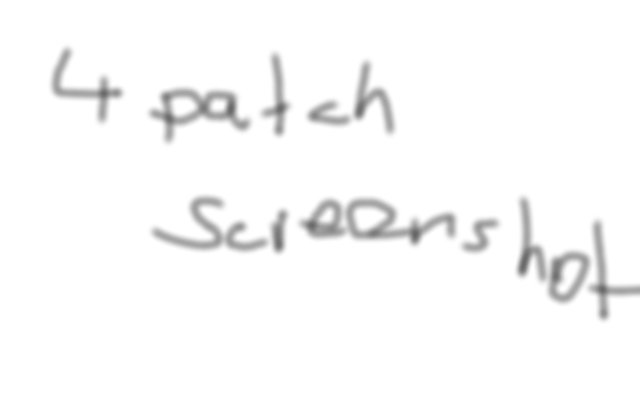
\includegraphics[width=\textwidth]{_raw_resources/4patch_composite.png}
	\caption{Actual order of computation}
	\label{fig:alt-render:4patch}
\end{figure}

Due to the system separation it is now possible to use green screen hardware 
compositor which have a visually higher quality in pulling the green background 
matte and then compositing it similarly into a mixed reality image. While this 
lifts some rendering overhead from the host PC, it fails in recreating a 
lightning environment for the VR actor and relies on two system. While engine 
programming complexity decreases, operational setup complexity increases.

\section{Rendering operational variations}
>>>>>>> Stashed changes

This setup can handle another operational context by leaving out 
background-sorting and only rendering a virtual "front", by which a high 
quality augmented camera setup can be achieved. Since time drift between camera 
and engine is already handled, it is possible to render an augmented image. 
Since depth information is lost, it is not possible to handle obstructions - in 
example by an interacting user that is standing in front of the augmented 
object. However, with some composition and choreography, AR footage can be 
showed and captured in live production for further use.
\newline
This thesis assumes that the motion video feed is calibrated for a D65 white 
and augmented reality scenarios usually do not take real world lightning into 
account, it would give a best, natural and high quality look into augmented 
reality showcases.

\section{Edge Cases}

The proposed method has edge cases which could be further improved by other 
approaches in rendering or capturing actor video. These highlight issues 
observed with the rendering operations discussed in this thesis.

\subsection{Image Clipping - incorrect Z calculation for hands}

Due to the planar projection of the real world feed inside the engine, any 
Z-information of the actor is squashed to a fixed point. This means that hands 
are on the same plane. In cases with high z-difference between actor and actors 
hands, it is possible that hand motion look unnatural and does not look like it 
is supposed - in figure [MISSING!] is an actor depicted, that wraps his arms 
around a virtual cube. The produced mixed reality image shows his arms only 
behind the cube.
\todo[inline]{add missing figure}
One solution for future research could be acquiring an actors depth by either 
using Time of Flight cameras and using a resulting point cloud or by 
calculating each camera pixels depth with stereoscopic setups. Thus each pixel 
could have a quantifiable depth with additional calibration parameters from the 
virtual reality tracking solution.

<<<<<<< Updated upstream
\subsection{Shadow Artifacts in multiple camera slices}

I believe I have solved that problem, but I gotta check.

\subsection{Culling Artifacts}

I zink' this is solved, too.
=======
\subsection{Matting failures}

There are multiple problems while green screening, which are as old as green 
screens are used in video production. First and foremost is a partial 
transparent actor if his clothing consists of similarly green shaded material.
\newline
Additional green screen spill causes artefacts while pulling the matte which 
then clips the actor off. This can be mitigated by better production 
environments, i. e. with higher quality cloth and a generally well lit set. 
\todo[inline]{"Proper Lightning Setup" should still be in the appendix :<}
Sometimes, for example in low light environments or folded green screen 
material, the background covers a wide color range, thus making a good 
calibration with a single color nearly impossible. This could be solved by 
smaller selection margins inside the shader while assigning an array of colors 
for the $\Delta E$ calculation. In turn, this would be even more taxing on the 
GPU.
\newline
Lastly, real time chroma keying has problems with motion blur of the source 
video material - causing background mixing and invalid matting. This is a 
complex problem that is far beyond the scope of this thesis.
\todo[inline]{Add graphics depicting each issue. Also cross reference to 
chapter 4}
>>>>>>> Stashed changes

\subsection{Calibration problems (wrong clipping, wrong reprojection, long 
setup times)}

The biggest margin of error is calibration of all projection parameters.
\newline
Beginning from field of view calculation, most DSLR cameras don't have 
specifications for their output feeds, where, for example, scaling factors 
could change the field of view angle. If these are not given or seem to be 
unfitting in production it is necessary to measure these parameters by hand, 
fixing the cameras position and calculating the spanning angle.
\todo[inline]{maybe add the ez calculation, too}
Another factor are offset-parameters between controllers and camera sensor, 
which have been minimized by the 3D printed attachment. However, minimal 
differences in this transformation matrix have tremendous impact on 
miscalculated projections, visible by wrongly placed objects and a disconnect 
between virtual interaction and actor.
\todo[inline]{Here comes a graphical representation of it}
Lastly, the most time spent after adding all mixed reality components to the 
scene is calibrating these parameters. A possible improvement could be done by 
fixing the cameras position, showing an overlay on the camera, where the 
secondary controller has to be placed and confirming it. This way the user can 
calibrate all projection parameters by himself with the help of a RANSAC / 
Lagrange Polynomial.
\todo[inline]{find out how this calibration is called: 
https://www.youtube.com/watch?v=c\_An0vxvPnk}